% !TEX root = ./ECEN-601 - Homework 2 - Brody Jordan.tex

\documentclass[11pt]{article}

\usepackage[
    assignmentDueDate={September 19, 2025 at 5:00 pm}
]{C:/Users/bljor/Sync/Courses/assignment}

\providecommand{\ra}{\rightarrow}
\renewcommand{\b}[1]{\ensuremath{\mathbf{#1}}}
\providecommand{\R}[1][]{\ensuremath{\mathbb{R}^{#1}}}
\usepackage{pgfplots}
\usetikzlibrary{calc}

\begin{document}
\makeAssignmentTitle

% ------ Problem 1 ------
\begin{homeworkProblem}
    Negate the following statement: For every real number $\varepsilon > 0$ there exists a positive integer $k$
    such that for all positive integers $n$, it is the case that $|a_n - k^2| < \varepsilon$. \vspace{1\baselineskip}

    \solution

    There exists some $\varepsilon > 0$ such that for each positive integer $k$, there exists some positive integer $n$ where $| a_n - k^2 | \geq \varepsilon$.

\end{homeworkProblem}

\pagebreak

% ------ Problem 2 ------
\begin{homeworkProblem}
    Let $f : X \ra Y$, $A, B \subseteq X$, and $C, D \subseteq Y$. Show that $f^{-1}$ preserves inclusions, unions,
    and intersections. \\[0.2\baselineskip]
    {[Hint: Recall that $f(A) \triangleq \{f(x) \mid x \in A\}$ and $f^{-1}(C) \triangleq \{x \in X \mid f(x) \in C\}$.]}
    \begin{enumerate}[label=(\alph*), itemsep=5pt, topsep=10pt]
        \item Show that $C \subseteq D \implies f^{-1}(C) \subseteq f^{-1}(D)$.
        \item Show that $f^{-1}(C \cup D) = f^{-1}(C) \cup f^{-1}(D)$.
        \item Show that $f^{-1}(C \cap D) = f^{-1}(C) \cap f^{-1}(D)$.
    \end{enumerate} \vspace{0.2\baselineskip}
    Show that $f$ preserves inclusions and unions, but not intersections.
    \begin{enumerate}[label=(\alph*), start=4, itemsep=5pt, topsep=10pt]
        \item Show that $A \subseteq B \Longrightarrow f(A) \subseteq f(B)$.
        \item Show that $f(A \cup B)=f(A) \cup f(B)$.
        \item Show that $f(A \cap B) \subseteq f(A) \cap f(B)$. Give an example where equality does not occur.
    \end{enumerate} \vspace{1\baselineskip}

    \solution

    \textbf{Part (a):} Say we have $x \in f^{-1}(C)$, then $f(x) \in C$, which implies $x \in C$. If we assume $C \subseteq D$, then $x \in D$, which
    means $f(x) \in D$, and if that is true, then $x \in f^{-1}(D)$. Thus, $f^{-1}(C) \subseteq f^{-1}(D)$. \\

    \textbf{Part (b):} Say we have $x \in f^{-1}(C \cup D)$, then $f(x) \in (C \cup D) \leftrightarrow f(x) \in C \cup f(x) \in D$. By the
    definition of the preimage, this means $x \in f^{-1}(C) \cup f^{-1}(D)$. Thus, $f^{-1}(C \cup D) = f^{-1}(C) \cup f^{-1}(D)$. \\

    \textbf{Part (c):} Say we have $x \in f^{-1}(C \cap D)$, then $f(x) \in (C \cap D) \leftrightarrow f(x) \in C \cap f(x) \in D$. By the
    definition of the preimage, this means $x \in f^{-1}(C) \cap f^{-1}(D)$. Thus, $f^{-1}(C \cap D) = f^{-1}(C) \cap f^{-1}(D)$. \\

    \textbf{Part (d):} Say we have $x \in A$, then $f(x) \in f(A)$. If we assume $A \subseteq B$, then $x \in B$, which means $f(x) \in f(B)$. Thus, $A \subseteq B \implies f(A) \subseteq f(B)$. \\

    \textbf{Part (e):} Say we have $x \in f(A \cup B)$, then $f(x) \in f(A \cup B)$, which means $f(x) \in f(A) \cup f(x) \in f(B)$. Thus, $f(A \cup B) = f(A) \cup f(B)$. \\

    \textbf{Part (d):} Say we have $x \in f(A \cap B)$, then $x \in A \cap B$. This means $f(x) \in f(A)$ and $f(x) \in f(B)$. Since $f(x)$ is in both sets, $f(A \cap B) \subseteq f(A) \cap f(B)$. \\

\end{homeworkProblem}

\pagebreak

% ------ Problem 3 ------
\begin{homeworkProblem}
    Let $\underline{x}=\left(x_1, \ldots, x_n\right)$,  $\underline{y}=\left(y_1, \ldots, y_n\right) \in \mathbb{R}^n$ and
    consider the function $\rho$ given by
    \[
        \rho(\underline{x}, \underline{y}) = \max{|x_1 - y_1|, \cdots, |x_n - y_n|}.
    \]
    Show that $\rho$ is a metric. \vspace{1\baselineskip}

    \solution

    In order for $\rho$ to be a metric, it must satisfy the following properties
    \begin{enumerate}[topsep=5pt, itemsep=2.5pt, ]
        \item $\rho(x, y) \geq 0 \quad \forall x, y \in X :$ \textit{equality holds if and only if} $x = y$
        \item $\rho(x, y) = \rho(y, x) \quad \forall x, y \in X$
        \item $\rho(x, y) + \rho(y, z) \geq \rho(x, z) \quad \forall x, y, z \in X$
    \end{enumerate}
    As stated in the problem, we are working over the real numbers. \\

    Starting from the top:
    \[
        \rho(\underline{x}, \underline{y}) = \max{|x_1 - y_1|, \cdots, |x_n - y_n|} \geq 0
    \]
    This inequality holds because we are taking the max of absolute values, so we will never get a negative number. Additionally, over the reals, we only
    get 0 when $x_i = y_i$. Thus, $\rho$ satisfies non-negativity. \\

    Next, we check if $\rho(\underline{x}, \underline{y}) = \rho(\underline{y}, \underline{x})$:
    \[
        \rho(\underline{x}, \underline{y}) = \max{|x_1 - y_1|, \cdots, |x_n - y_n|} = \max{|y_1 - x_1|, \cdots, |y_n - x_n|} = \rho(\underline{y}, \underline{x})
    \]
    We know this is true since $|a - b| = |b - a|$ for $a, b \in \R$. Thus, $\rho$ satisfies symmetry. \\

    Finally, the triangle inequality:
    \begin{align*}
        \rho(\underline{x}, \underline{y}) + \rho(\underline{y}, \underline{z})         & \geq \rho(\underline{x}, \underline{z})     \\
        \max{|x_1 - y_1|, \cdots, |x_n - y_n|} + \max{|y_1 - z_1|, \cdots, |y_n - z_n|} & \geq \max{|x_1 - z_1|, \cdots, |x_n - z_n|}
    \end{align*}
    Holds since $|x_k - z_k| = |(x_k - y_k) + (y_k - z_k)|$ and each term inside the absolute value is upper bounded by the maximum value. \\

    $\rho$ satisfies all three properties, so it is a metric.
\end{homeworkProblem}

\pagebreak

% ------ Problem 4 ------
\begin{homeworkProblem}
    Suppose $a \in B_d (x, \varepsilon)$ with $\varepsilon > 0$. Find an explicit $\delta > 0$ such that the open ball
    $B_d(a, \delta)$ centered at $a$ is contained in $B_d(x, \varepsilon)$. \vspace{1\baselineskip}

    \solution

    We have a set $B_d(x, \varepsilon) = \{y \in X \mid d(x, y) < \varepsilon\}$ in which we find $a$. This means that $d(x, a) < \varepsilon$. \\

    We need some $\delta$ such that $\forall y \in B_d(a, \delta)$, $y \in B_d(x, \varepsilon)$. \\

    I think this problem is very easy to solve visually:

    \begin{figure}[h!]
        \centering
        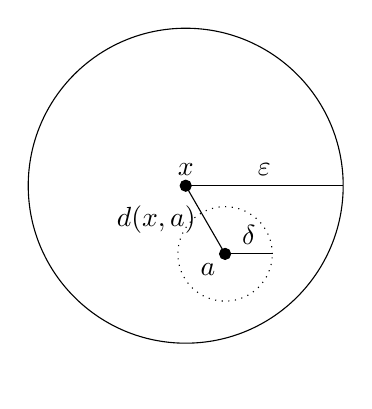
\begin{tikzpicture}[scale=2]

            \draw[fill=none](0,0) circle (1.0) node [black,yshift=-1.5cm] {};
            \draw[fill=black](0,0) circle (1 pt) node [above] {$x$};
            \draw[](0,0) -- (1,0) node [midway,above] {$\varepsilon$};
            \draw[](0,0) -- (0.25,-0.433) node [midway,left] {$d(x,a)$};
            % dot for a
            \draw[fill=black](0.25,-0.433) circle (1 pt) node [below left] {$a$};
            % draw dotted delta circle
            \draw[fill=none,dotted](0.25,-0.433) circle (0.3) node [black,yshift=-1.5cm] {};
            % draw line from a to edge of delta circle
            \draw[](0.25,-0.433) -- (0.55,-0.433) node [midway,above] {$\delta$};
        \end{tikzpicture}
    \end{figure}
    As we can see above, $\delta$ is simply less than the difference between $\varepsilon$ and $d(x, a)$.
    Thus, for any $\delta$ such that $\delta < \varepsilon - d(x, a)$, $B_d(a, \delta) \subset B_d(x, \varepsilon)$.
\end{homeworkProblem}

\pagebreak

% ------ Problem 5 ------
\begin{homeworkProblem}
    This problem outlines a proof that the Euclidean distance $d$ on $\mathbb{R}^n$ is a metric, as follows: If
    $\b{x}, \b{y} \in \mathbb{R}^n$ and $c \in \mathbb{R}$, define
    \begin{align*}
        \b{x} + \b{y}     & =\left(x_1+y_1, \ldots, x_n+y_n\right) & c \b{x}   & =\left(c x_1, \ldots, c x_n\right), \\
        \b{x} \cdot \b{y} & =x_1 y_1+\cdots+x_n y_n                & \|\b{x}\| & =(\b{x} \cdot \b{x})^{1 / 2} .
    \end{align*}
    \begin{enumerate}[label=(\alph*), itemsep=5pt]
        \item Show that $\b{x} \cdot (\b{y} + \b{z}) = (\b{x} \cdot \b{y}) + (\b{x} \cdot \b{z})$.
        \item Show that $|\b{x} \cdot \b{y}| \leq \norm{\b{x}} \norm{\b{y}}$. [Hint: if $\b{x}, \b{y} \neq 0$,
                      let $a = 1/\norm{\b{x}}$ and $b = 1/\norm{\b{y}}$, and use the fact that $\norm{a\b{x} \pm b \b{y}} \geq 0$.]
        \item Show that $\norm{\b{x} + \b{y}} \leq \norm{\b{x}} + \norm{\b{y}}$. [Hint: Compute $(\b{x} + \b{y}) \cdot (\b{x} + \b{y})$
                      and apply previous result.]
        \item Verify that the Euclidean distance $d(\b{x}, \b{y})$ is a metric.
    \end{enumerate} \vspace{1\baselineskip}

    \solution

    \textbf{Part (a):} Very simply,
    \begin{align*}
        \b{x} \cdot (\b{y} + \b{z}) & = x_1 (y_1 + z_1) + \cdots + x_n (y_n + z_n)                  \\
                                    & = x_1 y_1 + x_1 z_1 + \cdots + x_n y_n + x_n z_n              \\
                                    & = (x_1 y_1 + \cdots + x_n y_n) + (x_1 z_1 + \cdots + x_n z_n) \\
                                    & = (\b{x} \cdot \b{y}) + (\b{x} \cdot \b{z})                   \\
    \end{align*}
    \textbf{Part (b):} Let $a = 1/\norm{\b{x}}$ and $b = 1/\norm{\b{y}}$. Then,
    \begin{align*}
        0 \leq \norm{a \b{x} + b \b{y}}^2 & = (a \b{x} + b \b{y}) \cdot (a \b{x} + b \b{y})                                                                                          \\
                                          & = a^2 (\b{x} \cdot \b{x}) + 2ab (\b{x} \cdot \b{y}) + b^2 (\b{y} \cdot \b{y})                                                            \\
                                          & = a^2 \norm{\b{x}}^2 + 2ab (\b{x} \cdot \b{y}) + b^2 \norm{\b{y}}^2                                                                      \\
                                          & = \frac{\norm{\b{x}}^2}{\norm{\b{x}}^2} + \frac{2(\b{x} \cdot \b{y})}{\norm{\b{x}} \norm{\b{y}}} + \frac{\norm{\b{y}}^2}{\norm{\b{y}}^2} \\
                                          & = 2 + \frac{2(\b{x} \cdot \b{y})}{\norm{\b{x}} \norm{\b{y}}} \geq 0                                                                      \\
                                          & \rightarrow \frac{2(\b{x}\cdot\b{y})}{\norm{\b{x}} \norm{\b{y}}} \geq -2                                                                 \\
                                          & \rightarrow \b{x} \cdot \b{y} \geq -\norm{\b{x}} \norm{\b{y}}                                                                            \\
                                          & \rightarrow |\b{x} \cdot \b{y}| \leq \norm{\b{x}} \norm{\b{y}}                                                                           \\
    \end{align*}

    \pagebreak

    \textbf{Part (c):} Applying the suggested method,
    \begin{align*}
        \norm{\b{x} + \b{y}}^2 & = (\b{x} + \b{y}) \cdot (\b{x} + \b{y})                                                                                    \\
                               & = \b{x} \cdot \b{x} + 2 (\b{x} \cdot \b{y}) + \b{y} \cdot \b{y}                                                            \\
                               & = \norm{\b{x}}^2 + 2 (\b{x} \cdot \b{y}) + \norm{\b{y}}^2 \leq \norm{\b{x}}^2 + 2\norm{\b{x}}\norm{\b{y}} + \norm{\b{y}}^2 \\
                               & \implies \norm{\b{x} + \b{y}} \leq \norm{\b{x}} + \norm{\b{y}}                                                             \\                                                             \\
    \end{align*}
    \textbf{Part (d):} In order for $d$ to be a metric, it must be nonnegative, symmetric, and satisfy the triangle inequality. The
    definition of the Euclidean distance is
    \[
        d(\b{x}, \b{y}) = \norm{\b{x} - \b{y}} = \sqrt{(x_1 - y_1)^2 + \cdots + (x_n - y_n)^2}
    \]
    Squaring a real number always results in a nonnegative number, and the square root of a nonnegative
    number is also nonnegative. Thus, $d(\b{x}, \b{y}) \geq 0$. Additionally, $d(\b{x}, \b{y}) = 0$ if and only if $\b{x} = \b{y}$. \\

    Since $|a - b| = |b - a|$, order in the Euclidean distance does not matter. Therefore, $d$ is symmetric. \\

    Finally, we know
    \[
        d(\b{x}, \b{y}) = \norm{\b{x} - \b{y}} = \norm{(\b{x} - \b{z}) + (\b{z} - \b{y})} \leq \norm{\b{x} - \b{z}} + \norm{\b{z} - \b{y}} = d(\b{x}, \b{z}) + d(\b{z}, \b{y})
    \]
    Thus, $d$ satisfies the triangle inequality, and is a metric.
\end{homeworkProblem}

\pagebreak

% ------ Problem 6 ------
\begin{homeworkProblem}
    Define $f_n : [0, 1] \ra \R$ by the equation $f_n(x) = x^n$. Show that the sequence $\{f_n(x)\}$ converges for each $x \in [0, 1]$,
    but that the sequence $\{f_n\}$ does not converge uniformly. Recall that uniform convergence to $f$ on $[a, b]$ implies that,
    for any $\varepsilon > 0$, there exists an $N$ such that $|f_n(t) - f(t)| < \varepsilon$ for all $n > N$ and all $t \in [a, b]$. \\

    \solution

    For all values of $x \in [0, 1)$, it is apparent that $\lim_{n \to \infty} x^n = 0$. When $x = 1$, $\lim_{n \to \infty} 1^n = 1$. This gives
    \[
        f(x) = \lim_{n \to \infty} f_n(x) =
        \begin{cases}
            0, & x \in [0, 1), \\
            1, & x = 1.
        \end{cases}
    \]

    As we did in lecture, let's choose some $\varepsilon$ that obviously fail the uniform convergence test. Here the gap will be quite large, so we can
    choose virtually any $\varepsilon < 1$. I'll choose $\varepsilon = \frac{9}{16}$ (the day I'm writing this).
    \[
        |f_n(t) - \underset{\rightarrow 0 \in [0, 1)}{f(t)}| < \varepsilon \implies |t^n| < \frac{9}{16}
    \]
    Choosing $n = N + 1$,
    \[
        t = \left(\frac{9}{16}\right)^{\frac{1}{N+1}}
    \]
    Now
    \[
        |f_{N+1}(t)| = \left(\frac{9}{16}\right)^{\frac{N+1}{N+1}} = \frac{9}{16} \not< \frac{9}{16}
    \]
    Therefore, the sequence does not converge uniformly.

\end{homeworkProblem}

\end{document}
